\documentclass[]{beamer}


% \usepackage{CJKnumb}\usepackage{beamerthemesplit}

\mode<article>
{
  \usepackage{beamerbasearticle}
  \usepackage{fullpage}
  \usepackage{hyperref}
}

\usepackage{algorithm}
\usepackage{algorithmic}
\usepackage{appendixnumberbeamer}
\usepackage{color, colortbl}
\usepackage{amstext}
\usepackage{relsize}

%\usepackage{beamerthemesplit} 
%\usepackage{beamerthemeshadow}  
%\usepackage[width=2cm,dark,tab]{beamerthemesidebar}


% Setup appearance:

%\usetheme{Darmstadt}
\usefonttheme[onlylarge]{structurebold}
\setbeamerfont*{frametitle}{size=\normalsize,series=\bfseries}
\setbeamertemplate{navigation symbols}{}

\renewcommand\arraystretch{1.5}

% Standard packages

\usepackage[english]{babel}
%\usepackage[latin1]{inputenc}

\usepackage{epsf}
\usepackage{amsmath,amssymb}
\usepackage{graphicx}
\usepackage{tabularx}

% \usepackage[usenames,dvipsnames]{color}
\definecolor{shadow}{gray}{0.8}
\newcommand{\redc}[1]{{\color{red} #1}}
\newcommand{\bluec}[1]{{\color{blue} #1}}
\newcommand{\shadowc}[1]{{\color{shadow} #1}}
\newcommand{\blackc}[1]{{\color{black} #1}}
\newcommand{\whitec}[1]{{\color{white} #1}}
\definecolor{myyellow}{HTML}{FFB700}
\newcommand{\yellowc}[1]{{\color{myyellow} #1}}
\newcommand{\greenc}[1]{{\color{green} #1}}
\newcommand{\vect}[1]{\textbf{\textit{#1}}}
\newcommand{\dd}[1]{\textrm{d}}
\newcommand{\corr}{C^{(3)}}

\newcommand{\AT}{{\textrm{{AT}}}}
\newcommand{\EX}{{\textrm{AT}}}
\newcommand{\CG}{{\textrm{CG}}}
\newcommand{\HY}{{\textrm{HY}}}
\newcommand{\thf}{{\textrm{th}}}
\newcommand{\rdf}{{\textrm{rdf}}}
\newcommand{\rep}{{\textrm{rep}}}

\usepackage{amsfonts}
\newcommand{\tickYes}{\checkmark}
\usepackage{pifont}
\newcommand{\tickNo}{\hspace{1pt}\ding{55}}


\definecolor{MyGray}{gray}{0.85}

\usepackage{array}
\newcolumntype{L}[1]{>{\raggedright\let\newline\\\arraybackslash\hspace{0pt}}m{#1}}
\newcolumntype{C}[1]{>{\centering\let\newline\\\arraybackslash\hspace{0pt}}m{#1}}
\newcolumntype{R}[1]{>{\raggedleft\let\newline\\\arraybackslash\hspace{0pt}}m{#1}}


\usetheme{Boadilla}
% \usetheme{Copenhagen}
% \usetheme{Madrid}
% \usetheme{Singapore}


\begin{document}
\title[Grand-Canonical MD by AdResS]{
  Grand-Canonical-Like Molecular Dynamics  by Using an
  Adaptive-Resolution Technique
}
%
\author{Han Wang}
\institute[FUB] {
  Institute for Mathematics, Freie Universit\"at Berlin, Germany\\
  % Institut f\"ur Mathematik, Freie Universit\"at Berlin, Germany\\
\vskip 0.4cm
Joint with: Carsten Hartmann, Christof Sch\"utte, Luigi Delle Site}
\date[Sept. 2013]{11 September 2013\\ 246th ACS National Meeting}
\frame{\titlepage}

\begin{frame}{AdResS: an overview}
  \redc{AdResS} = \redc{Ad}aptive \redc{Res}olution \redc{S}imulation
  \begin{figure}
    \centering 
    \includegraphics[width=0.55\textwidth]{fig/system.example/example-1.eps}
    % 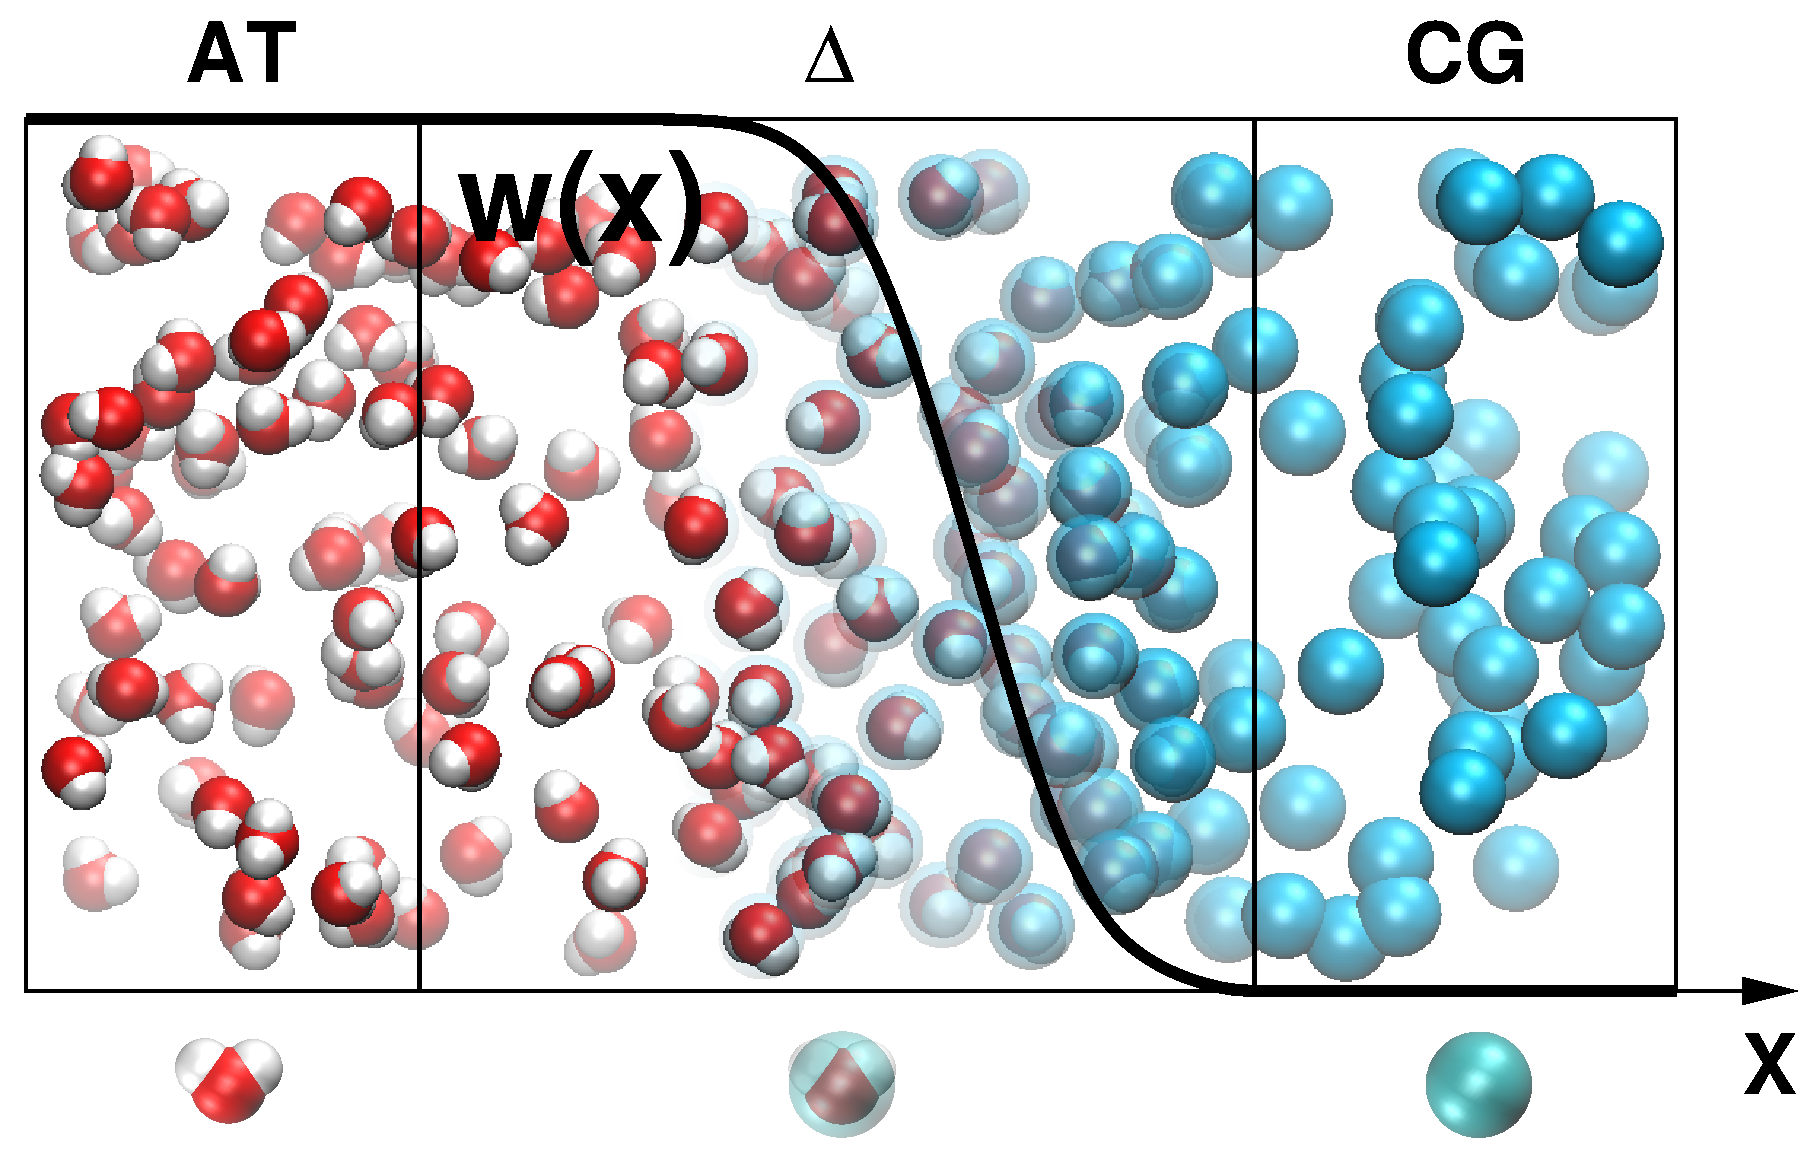
\includegraphics[width=0.8\textwidth]{fig/adapt-wat.eps}
  \end{figure}
  \footnotesize{B.P. Lambeth, Jr. \textit{et. al.} J. Chem. Phys. \textbf{133}, 221101 (2010)}
\end{frame}

\begin{frame}{Essential Principles}
  \vfill  
  \begin{enumerate}
  \item  \redc{Increase molecular resolution} in a subregion of the space
    keeping the rest of the system at a lower resolution.
  \item  Allow for the \redc{free exchange} of molecules from the
    high to the low resolution (and vice versa).
  \item  1 \& 2 \redc{must} occur under the conditions of {thermodynamic
      equilibrium} and structure consistency.
  \end{enumerate}
  \vfill
  \bluec{Advantages}:
  \begin{itemize}
  \item An optimal employment of \redc{computational resources}.
  \item Good \redc{accuracy} in catching the details of essential physics and
    chemistry.
  \end{itemize}
  \vfill
\end{frame}

\begin{frame}{AdResS: an overview}
  \redc{AdResS} = \redc{Ad}aptive \redc{Res}olution \redc{S}imulation
  \begin{figure}
    \centering 
    \includegraphics[width=0.55\textwidth]{fig/system.example/example-2.eps}
    % 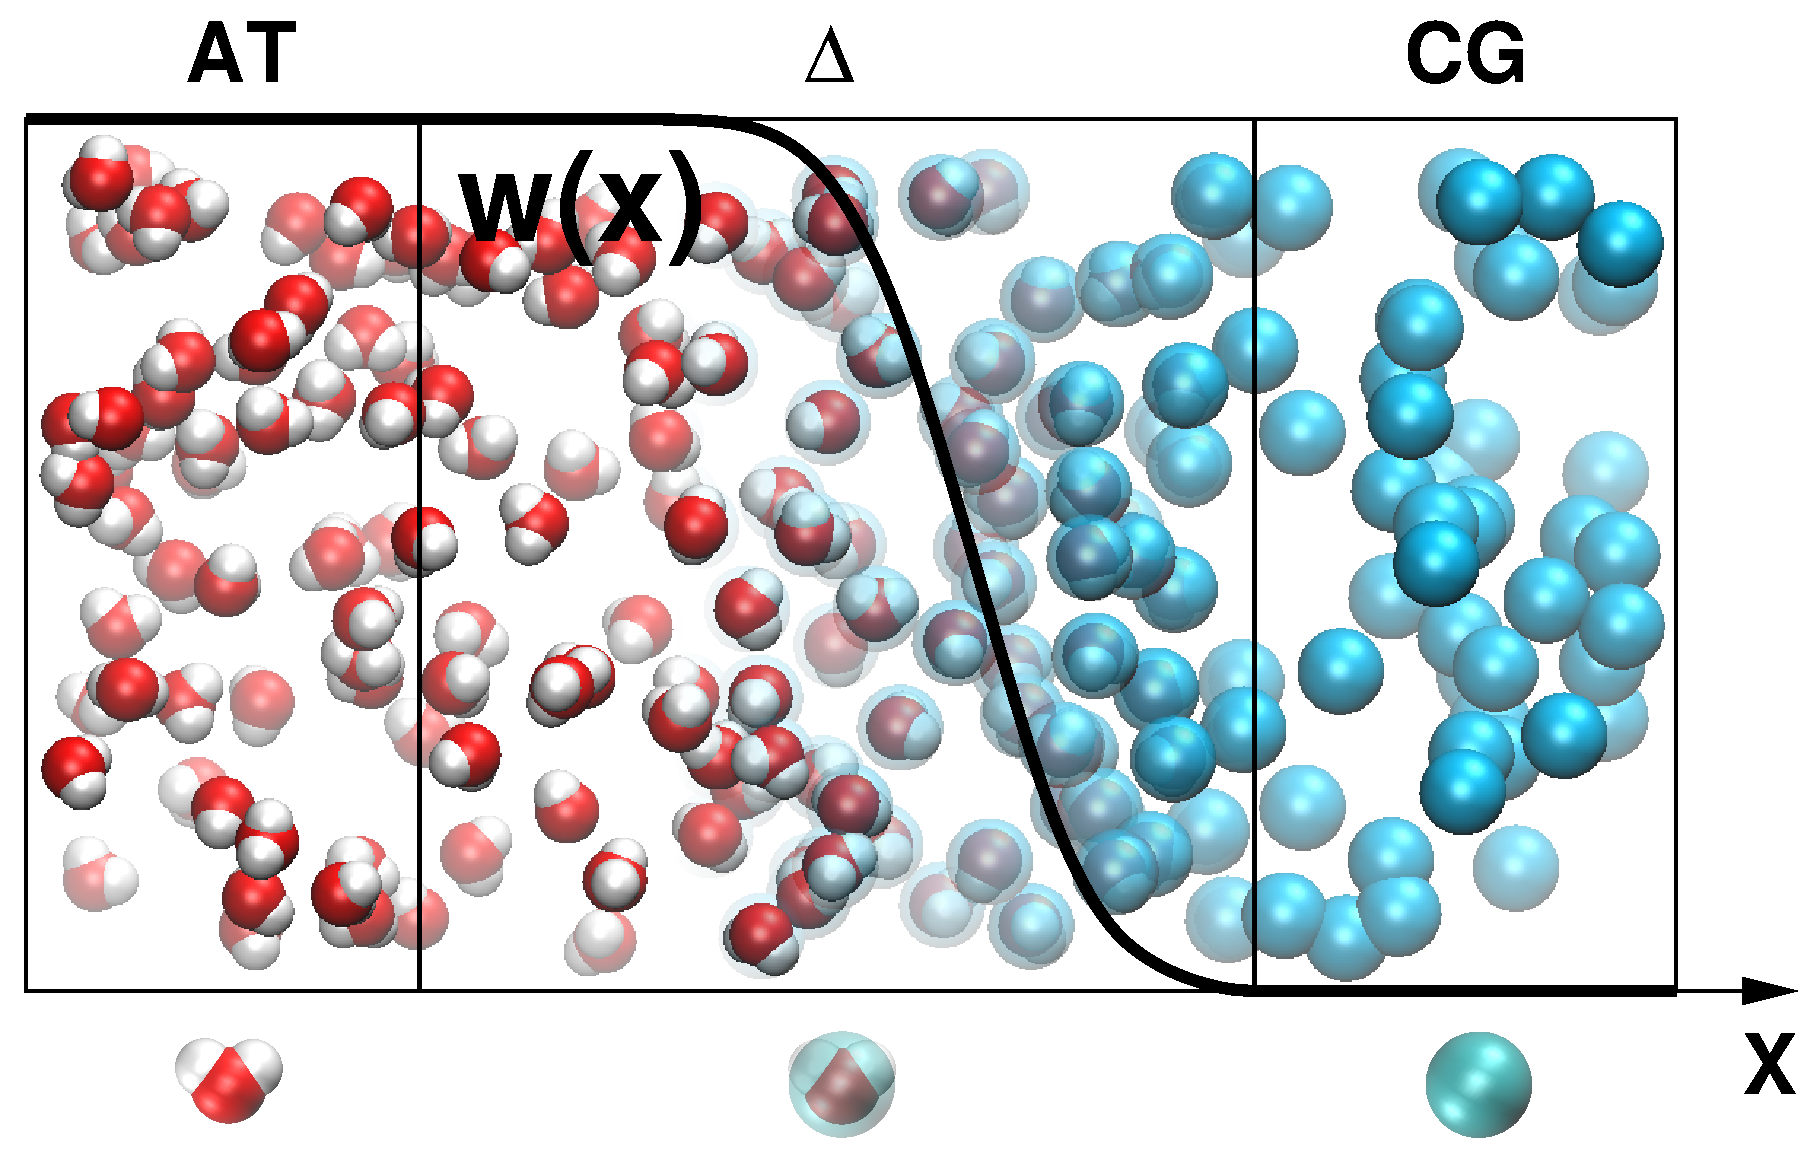
\includegraphics[width=0.8\textwidth]{fig/adapt-wat.eps}
  \end{figure}  
  \footnotesize{\whitec{B.P. Lambeth, Jr. \textit{et. al.} J. Chem. Phys. \textbf{133}, 221101 (2010)}}
\end{frame}


\begin{frame}{AdResS: an overview}
  \begin{itemize}
  \item <1-> The weighting function $w(x)$.
  \vskip -.1cm
  \begin{figure}
    \centering 
    \includegraphics[width=0.5\textwidth]{fig/system/system-neww.eps}
    % 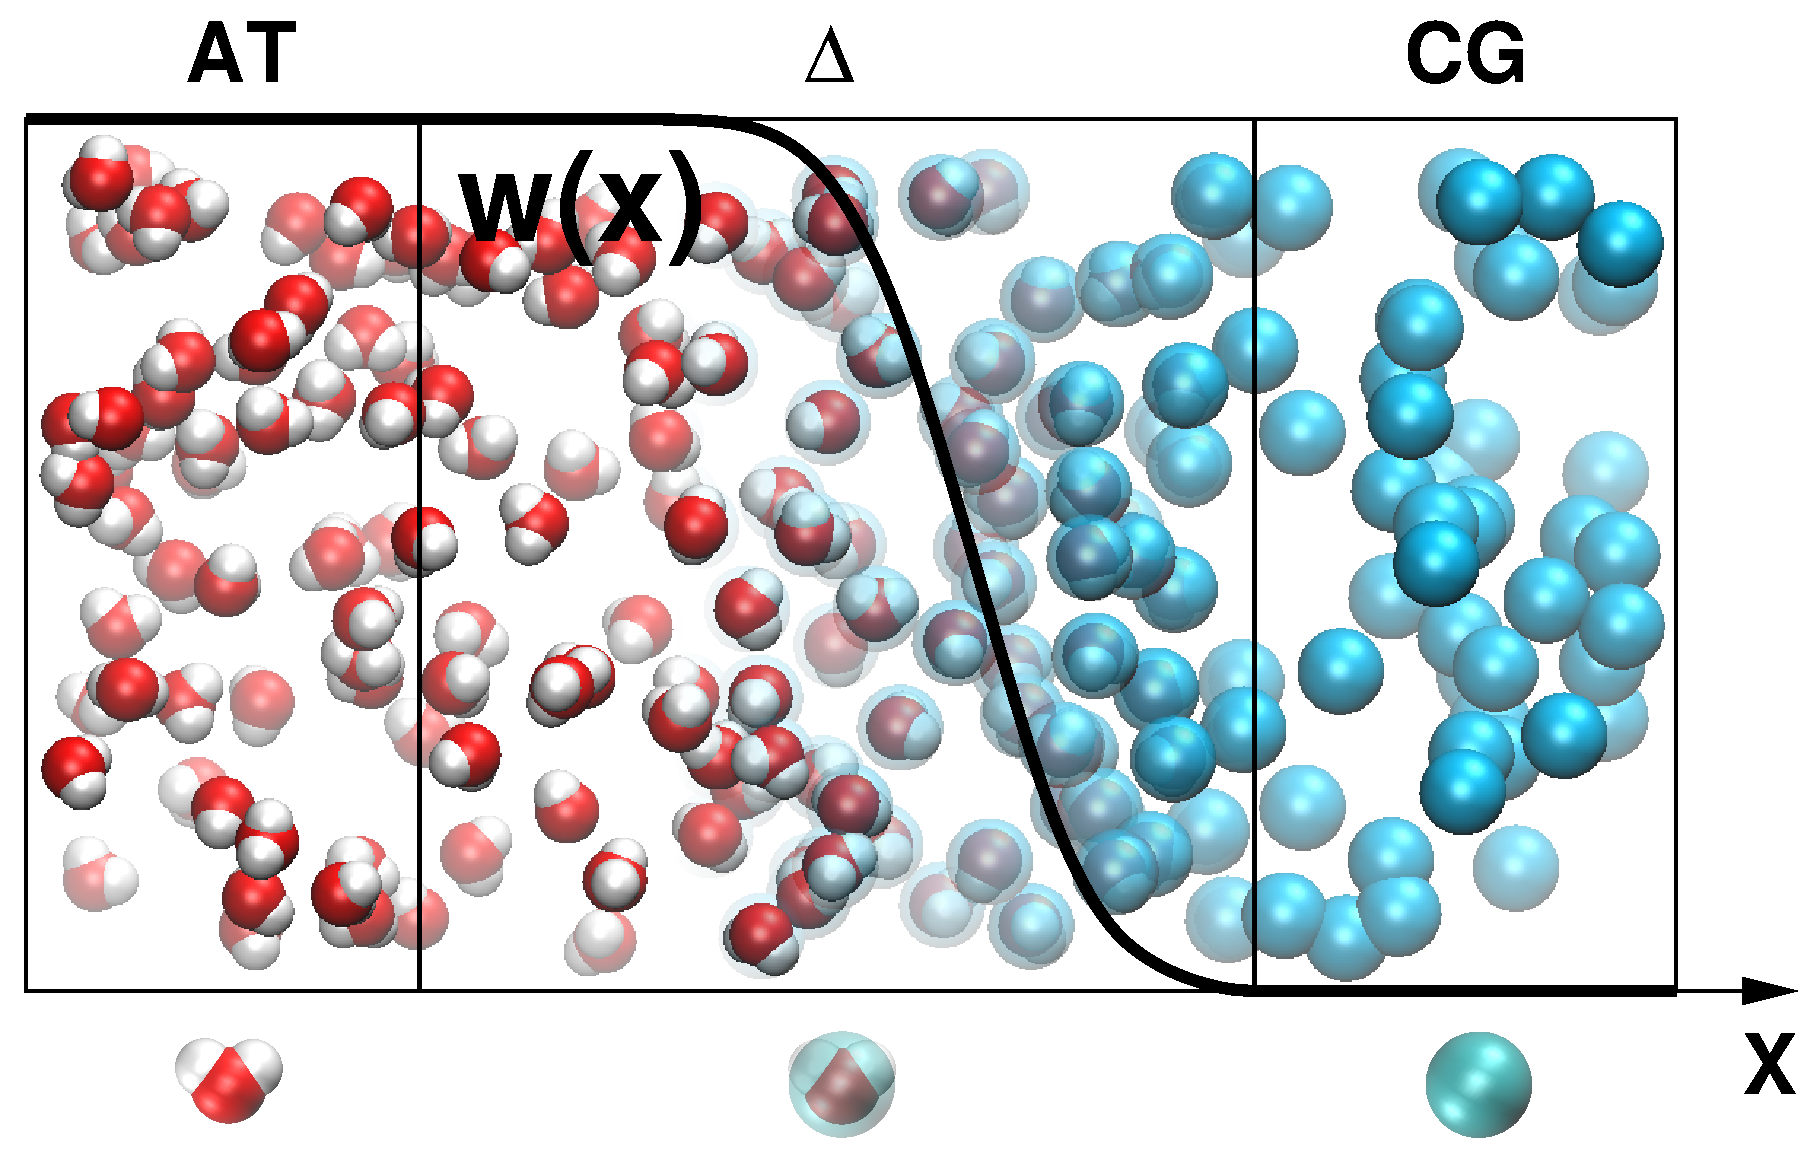
\includegraphics[width=0.8\textwidth]{fig/adapt-wat.eps}
  \end{figure}
  \vskip -.3cm
  \item<2-> Force interpolation scheme:
    \vskip -.6cm
  \begin{align*}
    {\vect F}_{\alpha \beta}&=w_\alpha w_\beta{\vect F}_{\alpha\beta}^{\AT}+[1-w_\alpha w_\beta]{\vect F}^{\CG}_{\alpha\beta} \whitec{\:+\: w_\alpha w_\beta (1-w_\alpha w_\beta)\vect F_{\alpha\beta}^{\rdf}}\\
    {\vect F}_{\alpha }& = \sum_{\beta}{\vect F}_{\alpha \beta} \whitec{\:+\:\vect F^\thf_{\alpha}}
  \end{align*}
  \end{itemize}
  % \footnote{M. Praprotnik, L. Delle Site, K. Kremer, JCP \textbf{123}, 224106 (2005)}
  \whitec{\footnotesize{S. Fritsch, \textit{et. al}
    \textbf{Phys. Rev. Lett.}, 108, (2012)}}\\
  \whitec{\footnotesize{H. Wang, C. Sch\"utte and L. Delle Site,
    \textbf{J. Chem. Theory \& Compt.}, 8(8), (2012)}}
\end{frame}


\begin{frame}{AdResS: an overview}
  \addtocounter{framenumber}{-1}
  \begin{itemize}
  \item <1-> The weighting function $w(x)$.
  \vskip -.1cm
  \begin{figure}
    \centering 
    \includegraphics[width=0.5\textwidth]{fig/system/system-neww.eps}
    % 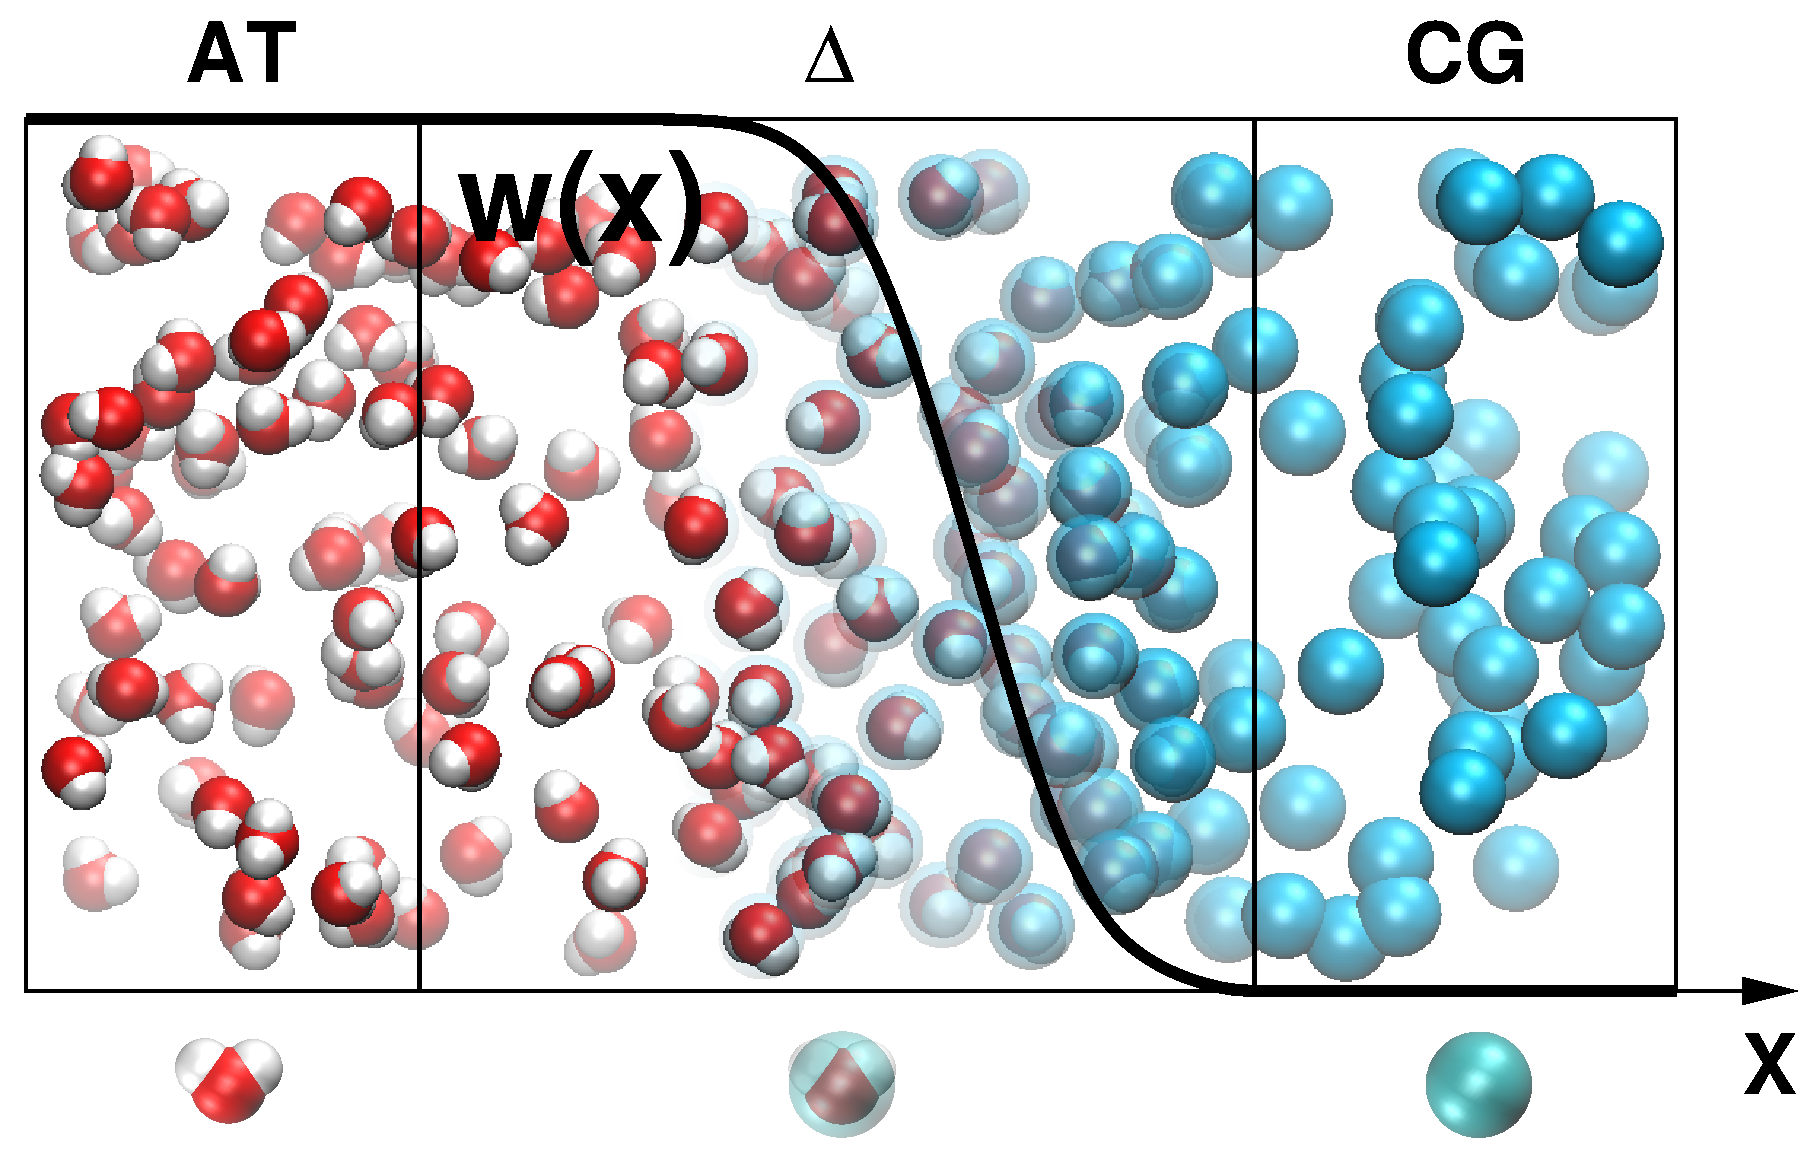
\includegraphics[width=0.8\textwidth]{fig/adapt-wat.eps}
  \end{figure}
  \vskip -.3cm
  \item<1-> Force interpolation scheme:
    \vskip -.6cm
  \begin{align*}
    {\vect F}_{\alpha \beta}&=w_\alpha w_\beta{\vect F}_{\alpha\beta}^{\AT}+[1-w_\alpha w_\beta]{\vect F}^{\CG}_{\alpha\beta} \bluec{\:+\: w_\alpha w_\beta (1-w_\alpha w_\beta)\vect F_{\alpha\beta}^{\rdf}}\\
    {\vect F}_{\alpha }& = \sum_{\beta}{\vect F}_{\alpha \beta} \bluec{\:+\:\vect F^\thf_{\alpha}}
  \end{align*}
  \end{itemize}
  {\footnotesize{S. Fritsch, \textit{et. al.},
    \textbf{Phys. Rev. Lett.}, 108, (2012)}}\\
  {\footnotesize{H. Wang, C. Sch\"utte and L. Delle Site,
    \textbf{J. Chem. Theory \& Compt.}, 8(8), (2012)}}
  % \footnote{M. Praprotnik, L. Delle Site, K. Kremer, JCP \textbf{123}, 224106 (2005)}
\end{frame}


\begin{frame}{AdResS: grand-canonical-like MD simulation}
    \vfill
  \begin{figure}
    \centering 
    \includegraphics[width=0.5\textwidth]{fig/system/partition.eps}
    % 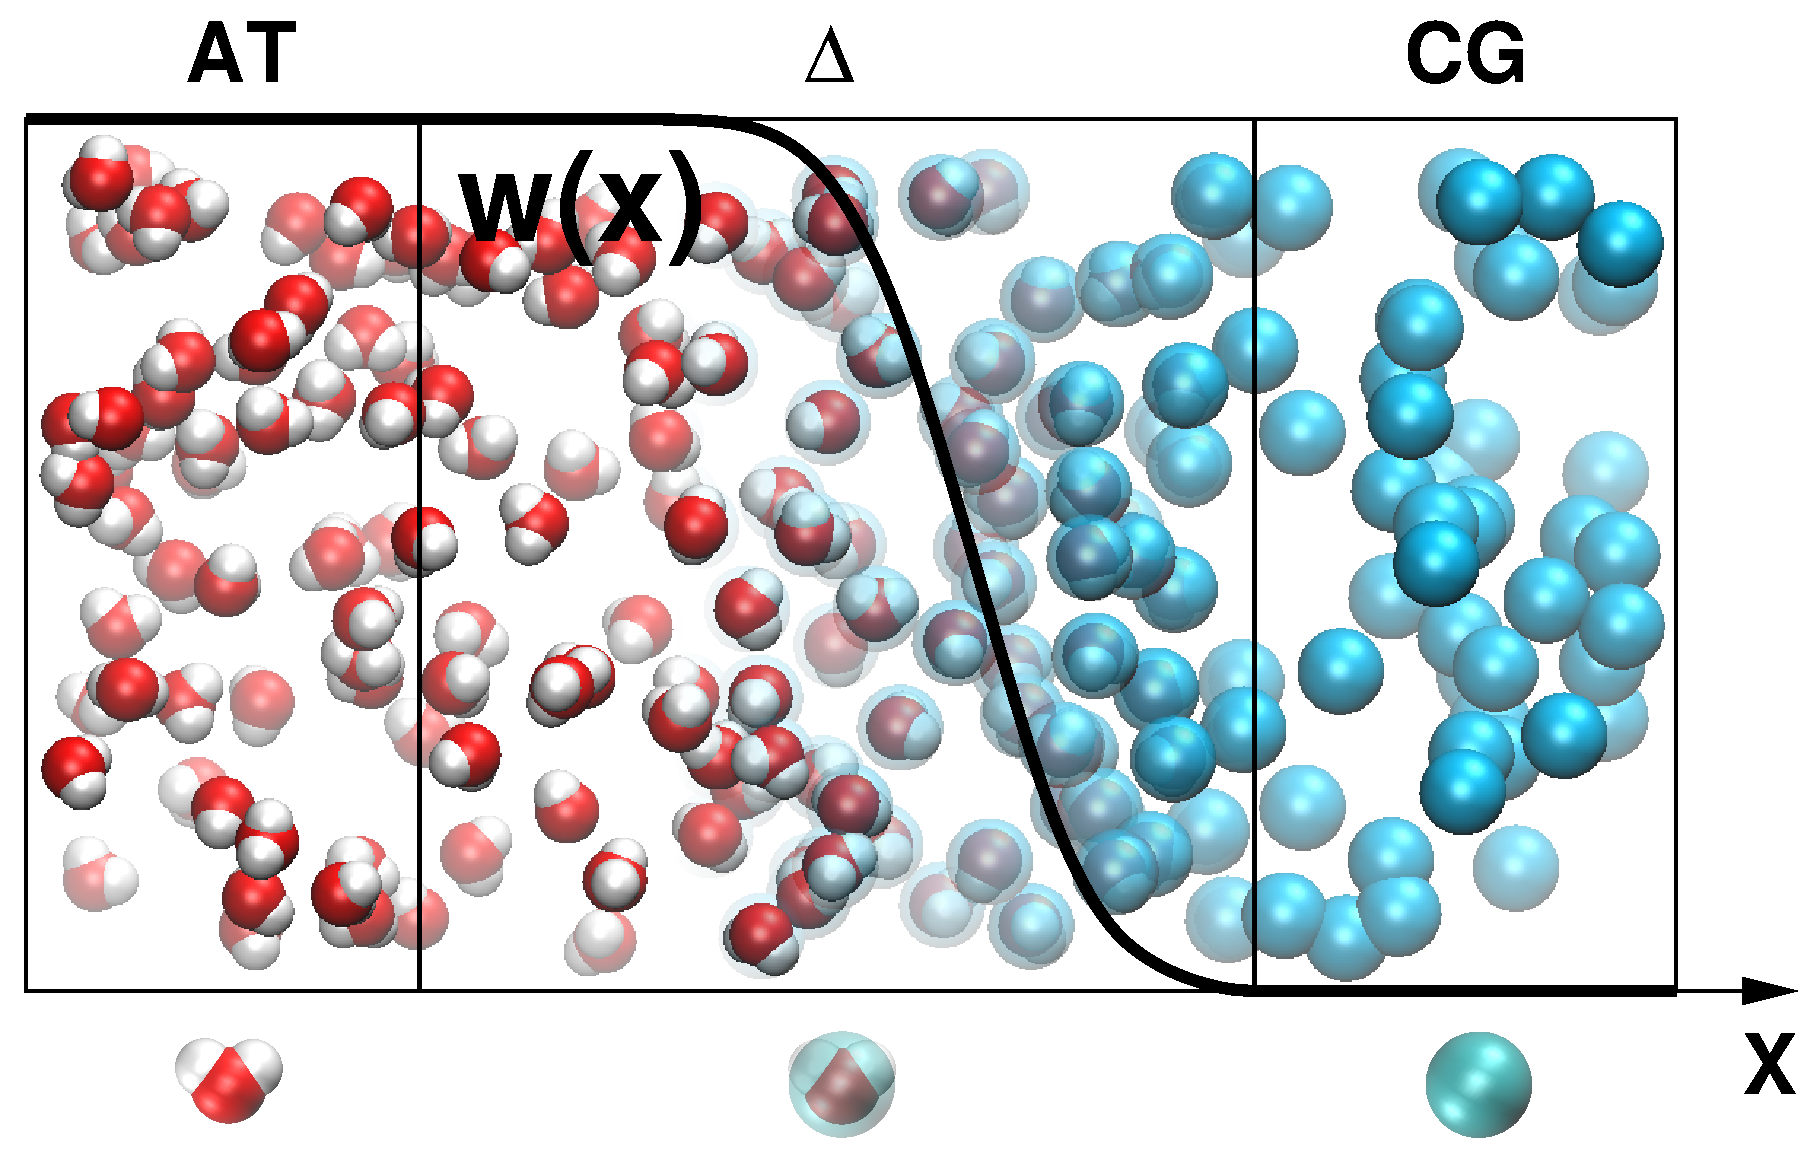
\includegraphics[width=0.8\textwidth]{fig/adapt-wat.eps}
  \end{figure}
  \begin{itemize}
    \vfill
  \item<1-> High-resolution region: system of interest.
    \vfill
  \item<2-> Low-resolution region: infinitly large particle reservior.
    \vfill
  \item<3-> Hybrid-resolution region: infinitly thin filter.
    \vfill
  \item <4-> Large enough system:
    \bluec{
      \begin{align*}
        N_\CG \gg 1,\qquad
        N_\AT \gg 1,\qquad
        N_\CG \gg N_\AT \gg N_\HY
      \end{align*}
    }
  \end{itemize}
    \vfill
\end{frame}


\begin{frame}{AdResS: grand-canonical-like MD simulation}  
  \vfill
  \begin{itemize}\itemsep .4cm
  \item <1->
    \bluec{Do we have the grand-canonical distribution?}
  \vfill
  \redc{
    \begin{align*}
      \mathlarger{\mathlarger{\mathlarger{
      p(\vect x_\AT, N_\AT) = \frac{1}{\mathcal Z_\EX}
      e^{\beta\mu_{\EX} N_\AT - \beta \mathcal H^{\EX}(\vect x_\AT)} }}}
    \end{align*}
  }      
  \vfill
  \item<2-> \bluec{$\mathcal Z_\EX$}: the partition function.
  \item<3-> \bluec{$\mu_{\EX}$}: the chemical potential of explicit reolution.
  \item<4-> \bluec{$\mathcal H^{\EX}$}: the explicit Hamiltonian.
  \end{itemize}
  \vfill
\end{frame}


\begin{frame}{AdResS: grand-canonical-like MD simulation}
  \begin{itemize}
    % \item<1-> Do we have the grand-canonical distribution?
    %   \bluec{
    %   \begin{align*}
    %     p(\vect x_\AT, N_\AT) = \frac{1}{\mathcal Z_\EX}
    %     e^{\beta\mu_{EX} N_\AT - \beta \mathcal H^{EX}(\vect x_\AT)} 
    %   \end{align*}}
  \item <1-> Decomposition:
    \bluec{
      \begin{align*}
        p(\vect x_\AT, N_\AT) = p(\vect x_\AT \vert N_\AT) \,{p (N_\AT)}
      \end{align*}}
  \item <2-> A step further:
    \bluec{
      \begin{align*}
        p(\vect x_\AT \vert N_\AT) =
        \sum_{N_\HY} \int \textrm{d}\vect x_\HY\,
        p(\vect x_\AT \vert N_\AT; \vect x_\HY, N_\HY)\cdot
        p(\vect x_\HY, N_\HY\vert N_\AT)
      \end{align*}
    }
  % \item <3-> By ideally ``freezing'' the DOFs \bluec{$\vect x_\HY, N_\HY$}, we have:
  %   \bluec{
  %     \begin{align*}
  %       p(\vect x_\AT \vert N_\AT; \vect x_\HY, N_\HY) \propto&
  %       e^{-\beta \mathcal H^\EX_{N_\AT}(\vect x_\AT; \vect x_\HY, N_\HY)}\\
  %       \mathcal H^\EX_{N_\AT}(\vect x_\AT; \vect x_\HY, N_\HY) 
  %       =&
  %       {\mathsmaller{
  %           \sum_{i=1}^{N_\AT}\frac12 m_i\vect v_i^2 +
  %           \sum_{i<j}^{N_\AT}U^\EX(\vect r_i - \vect r_j) }}\\
  %       &+ \mathsmaller{
  %       \sum_{i=1}^{N_\AT}\sum_{j=N_\AT+1}^{N_\AT + N_\HY}U^\EX(\vect r_i - \vect r_j)}
  %     \end{align*}
  %   }
  \end{itemize}
\end{frame}


\begin{frame}{AdResS: grand-canonical-like MD simulation}
  \begin{itemize}
    \vfill
  \item <1-> Consider \bluec{$p(\vect x_\AT \vert N_\AT; \vect x_\HY, N_\HY)$}.
    \vfill
  \item <2-> Electrostatic: Reaction field method.
    \vfill
  \item <3->
     ``\bluec{$\AT$}''  is interacting with
    ``\bluec{$\HY$}'' in an atomistic way.\\
    ``\bluec{$\CG$}''  is interacting with
    ``\bluec{$\HY$}'' in an coarse-grained way.
    \vfill
  \item <4-> By ideally ``freezing'' the DOFs \bluec{$\vect x_\HY, N_\HY$}, we have:
    \bluec{
      \begin{align*}
        p(\vect x_\AT \vert N_\AT; \vect x_\HY, N_\HY) \propto&
        \exp\{-\beta \mathcal H^\EX_{N_\AT}(\vect x_\AT; \vect x_\HY, N_\HY)\}
      \end{align*}
    }
    with
    \bluec{
      \begin{align*}
        \mathcal H^\EX_{N_\AT}(\vect x_\AT; \vect x_\HY, N_\HY) 
        =&
        {\mathsmaller{
            \sum_{i=1}^{N_\AT}\frac12 m_i\vect v_i^2 +
            \sum_{i<j}^{N_\AT}U^\EX(\vect r_i - \vect r_j) }}\\
        &+ \mathsmaller{
        \sum_{i=1}^{N_\AT}\sum_{j=N_\AT+1}^{N_\AT + N_\HY}U^\EX(\vect r_i - \vect r_j)}
      \end{align*}
    }
    \vfill
  \end{itemize}
\end{frame}


\begin{frame}{AdResS: grand-canonical-like MD simulation}
  \begin{minipage}[t][8cm][t]{1.0\linewidth}
    \begin{figure}[t]
      \centering
      \includegraphics[width=0.8\textwidth]{fig/traj.statistic/frame-00.eps}
    \end{figure}
  \end{minipage}
\end{frame}

\begin{frame}{AdResS: grand-canonical-like MD simulation}
  \addtocounter{framenumber}{-1}
  \begin{minipage}[t][8cm][t]{1.0\linewidth}
    \begin{figure}[t]
      \centering
      \includegraphics[width=0.8\textwidth]{fig/traj.statistic/frame-01.eps}
    \end{figure}
  \end{minipage}
\end{frame}

\begin{frame}{AdResS: grand-canonical-like MD simulation}
  \addtocounter{framenumber}{-1}
  \begin{minipage}[t][8cm][t]{1.0\linewidth}
    \begin{figure}[t]
      \centering
      \includegraphics[width=0.8\textwidth]{fig/traj.statistic/frame-02.eps}
    \end{figure}
  \end{minipage}
\end{frame}

\begin{frame}{AdResS: grand-canonical-like MD simulation}
  \addtocounter{framenumber}{-1}
  \begin{minipage}[t][8cm][t]{1.0\linewidth}
    \begin{figure}[t]
      \centering
      \includegraphics[width=0.8\textwidth]{fig/traj.statistic/frame-03.eps}
    \end{figure}
  \end{minipage}
\end{frame}


\begin{frame}{AdResS: grand-canonical-like MD simulation}
  \addtocounter{framenumber}{-1}
  \begin{minipage}[t][8cm][t]{1.0\linewidth}
    \begin{figure}[t]
      \centering
      \includegraphics[width=0.8\textwidth]{fig/traj.statistic/frame-10.eps}
    \end{figure}
  \end{minipage}
\end{frame}

\begin{frame}{AdResS: grand-canonical-like MD simulation}
  \addtocounter{framenumber}{-1}
  \begin{minipage}[t][8cm][t]{1.0\linewidth}
    \begin{figure}[t]
      \centering
      \includegraphics[width=0.8\textwidth]{fig/traj.statistic/frame-11.eps}
    \end{figure}
  \end{minipage}
\end{frame}

\begin{frame}{AdResS: grand-canonical-like MD simulation}
  \addtocounter{framenumber}{-1}
  \begin{minipage}[t][8cm][t]{1.0\linewidth}
    \begin{figure}[t]
      \centering
      \includegraphics[width=0.8\textwidth]{fig/traj.statistic/frame-12.eps}
    \end{figure}
  \end{minipage}
\end{frame}

\begin{frame}{AdResS: grand-canonical-like MD simulation}
  \addtocounter{framenumber}{-1}
  \begin{minipage}[t][8cm][t]{1.0\linewidth}
    \begin{figure}[t]
      \centering
      \includegraphics[width=0.8\textwidth]{fig/traj.statistic/frame-13.eps}
    \end{figure}
  \end{minipage}
\end{frame}

\begin{frame}{AdResS: grand-canonical-like MD simulation}
  \addtocounter{framenumber}{-1}
  \begin{minipage}[t][8cm][t]{1.0\linewidth}
    \begin{figure}[t]
      \centering
      \includegraphics[width=0.8\textwidth]{fig/traj.statistic/frame-20.eps}
    \end{figure}
  \end{minipage}
\end{frame}

\begin{frame}{AdResS: grand-canonical-like MD simulation}
  \addtocounter{framenumber}{-1}
  \begin{minipage}[t][8cm][t]{1.0\linewidth}
    \begin{figure}[t]
      \centering
      \includegraphics[width=0.8\textwidth]{fig/traj.statistic/frame-21.eps}
    \end{figure}
  \end{minipage}
\end{frame}

\begin{frame}{AdResS: grand-canonical-like MD simulation}
  \addtocounter{framenumber}{-1}
  \begin{minipage}[t][8cm][t]{1.0\linewidth}
    \begin{figure}[t]
      \centering
      \includegraphics[width=0.8\textwidth]{fig/traj.statistic/frame-22.eps}
    \end{figure}
  \end{minipage}
\end{frame}

\begin{frame}{AdResS: grand-canonical-like MD simulation}
  \addtocounter{framenumber}{-1}
  \begin{minipage}[t][8cm][t]{1.0\linewidth}
    \begin{figure}[t]
      \centering
      \includegraphics[width=0.8\textwidth]{fig/traj.statistic/frame-23.eps}
    \end{figure}
  \end{minipage}
\end{frame}

\begin{frame}{AdResS: grand-canonical-like MD simulation}
  \addtocounter{framenumber}{-1}
  \begin{minipage}[t][8cm][t]{1.0\linewidth}
    \begin{figure}[t]
      \centering
      \includegraphics[width=0.8\textwidth]{fig/traj.statistic/frame-24.eps}
    \end{figure}
  \end{minipage}
\end{frame}

\begin{frame}{AdResS: grand-canonical-like MD simulation}
  \begin{itemize}
  \item <1-> Reminder:
    \bluec{
      \begin{align*}
        p(\vect x_\AT \vert N_\AT) =
        \sum_{N_\HY} \int \textrm{d}\vect x_\HY\,
        p(\vect x_\AT \vert N_\AT; \vect x_\HY, N_\HY)\cdot
        p(\vect x_\HY, N_\HY\vert N_\AT)
      \end{align*}
      }
  \item <1-> After considering all possible combinations of
    \bluec{$N_\AT, N_\HY, \vect x_\HY$}:
    \bluec{
      \begin{align*}
        p(\redc{\vect x_\AT} \vert N_\AT; \vect x_\HY, N_\HY) \propto&
        \exp\{-\beta\, \mathcal H^\EX_{N_\AT}(\redc{\vect x_\AT}; \vect x_\HY, N_\HY)\}
      \end{align*}
    }
  \item <2-> Now the configuration in ``\bluec{$\HY$}''.
    \bluec{
      \begin{align*}
        p(\vect x_\HY, N_\HY\vert N_\AT) = \textrm{\huge{?}}
      \end{align*}
    }
  \end{itemize}
\end{frame}


\begin{frame}{AdResS: grand-canonical-like MD simulation}
  \hfill
  \begin{minipage}[c]{0.60\linewidth}
    \begin{figure}
      \centering 
      \includegraphics[width=0.80\textwidth]{fig/system/at-equiv.eps}
      % 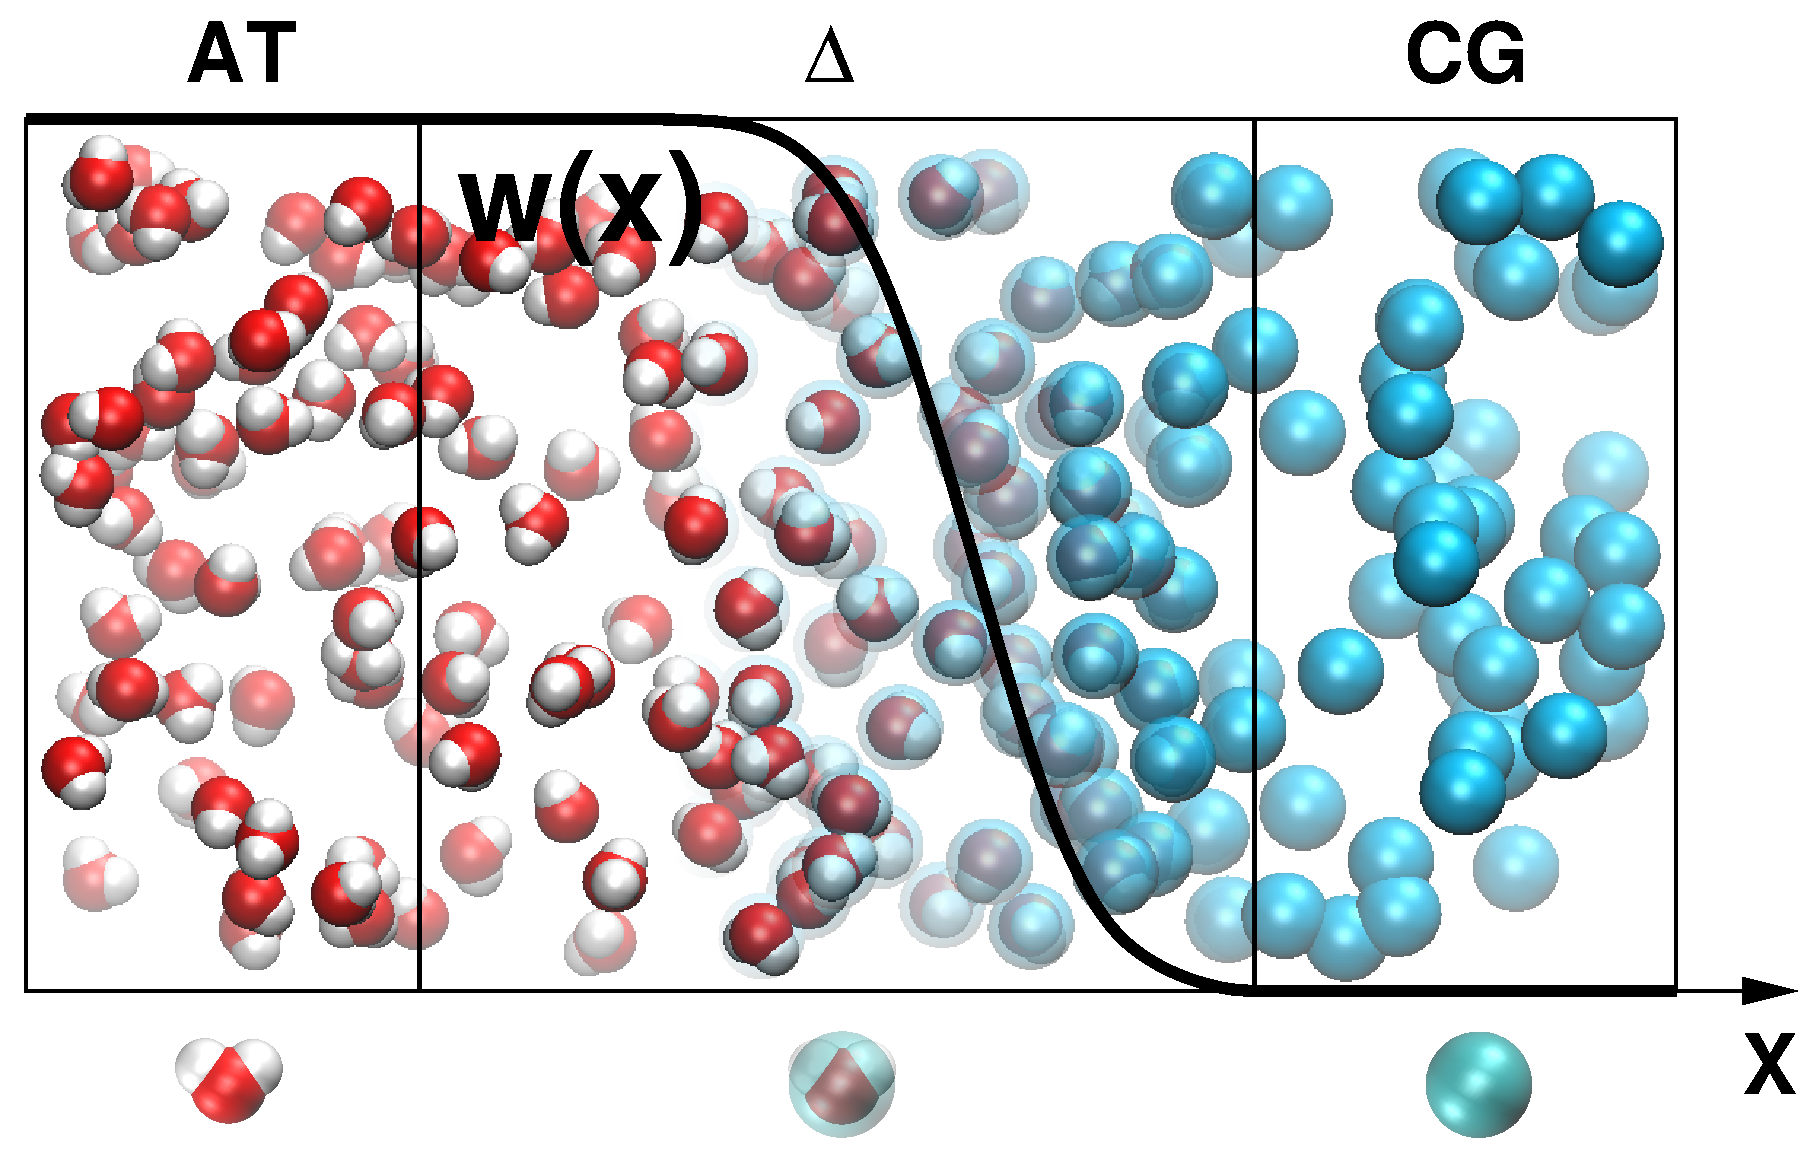
\includegraphics[width=0.8\textwidth]{fig/adapt-wat.eps}
    \end{figure}      
  \end{minipage}
  \hfill
  \begin{minipage}[c]{0.34\linewidth}
    % \small{Accuracy of} \bluec{$p(\vect x_\AT | N_\AT) $}\\
    % \small{Accuracy of configuration in the hybrid region}\\
    \vfill
    \whitec{
    Necessary conditions\\
    First order:\\
    {$\rho_{\HY} = \rho_\EX$}\\
    {\footnotesize{Thermodynamics force}}
    \vskip .2cm
    Second order:\\
    {$g_{\HY}(r) = g_\EX(r)$}\\
    {\footnotesize{RDF correction}}
    \vskip .2cm
    Third order:\\
    {$\corr_\HY = \corr_\AT$}\\
    {\footnotesize{Numerically verified}}
    \vskip .2cm
    Systematic improvement
    }
  \end{minipage}
  \hfill
\end{frame}

\begin{frame}{AdResS: grand-canonical-like MD simulation}
  \addtocounter{framenumber}{-1}
  \hfill
  \begin{minipage}[c]{0.60\linewidth}
    \begin{figure}
      \centering 
      \includegraphics[width=0.80\textwidth]{fig/system/at-equiv.eps}
      % 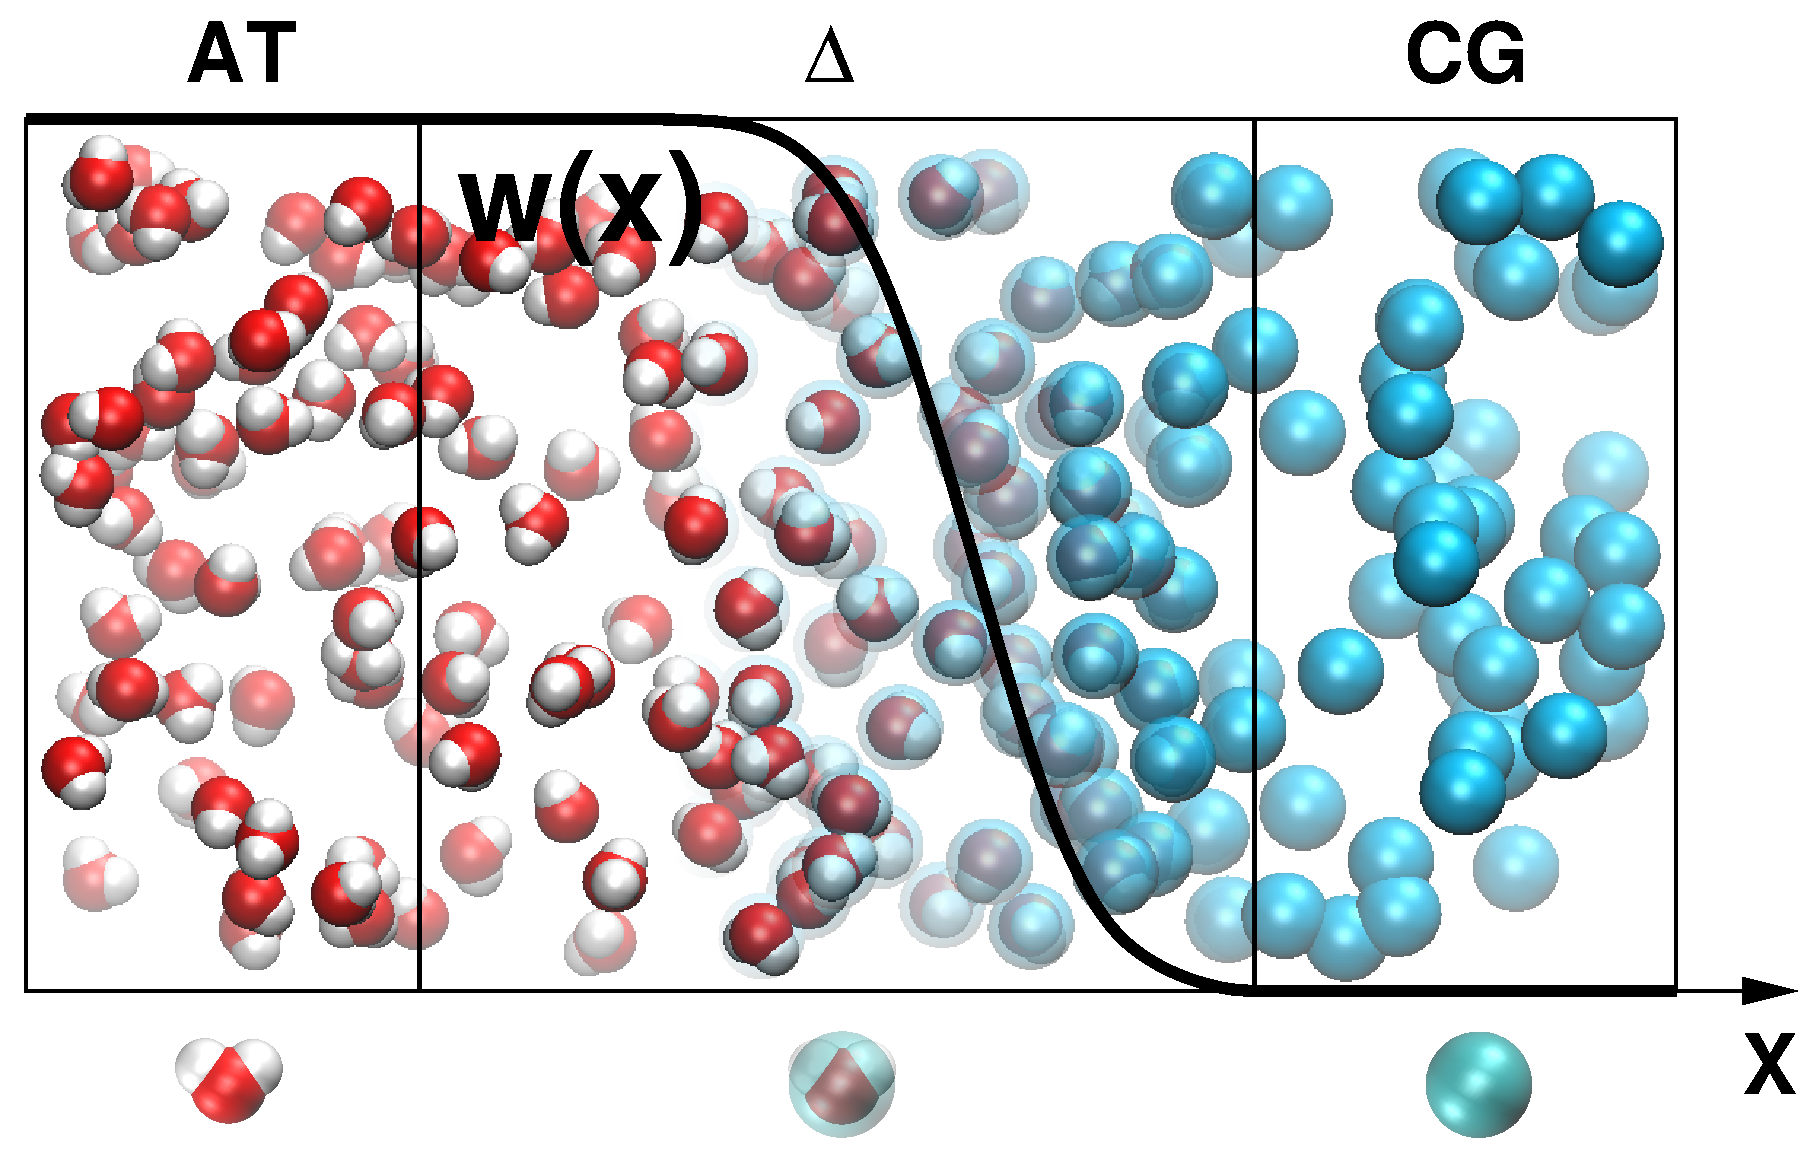
\includegraphics[width=0.8\textwidth]{fig/adapt-wat.eps}
    \end{figure}      
  \end{minipage}
  \hfill
  \begin{minipage}[c]{0.34\linewidth}
    % \small{Accuracy of} \bluec{$p(\vect x_\AT | N_\AT) $}\\
    % \small{Accuracy of configuration in the hybrid region}\\
    \vfill
    Necessary conditions\\
    First order:\\
    \bluec{$\rho_{\HY} = \rho_\EX$}\\
    \redc{\footnotesize{Thermodynamics force}}
    \vskip .2cm
    Second order:\\
    \bluec{$g_{\HY}(r) = g_\EX(r)$}\\
    \redc{\footnotesize{RDF correction}}
    \vskip .2cm
    Third order:\\
    \bluec{$\corr_\HY = \corr_\EX$}\\
    \redc{\footnotesize{Numerically verified}}
    \vskip .2cm
    Systematic improvement
  \end{minipage}
  \hfill
\end{frame}

\begin{frame}{AdResS: grand-canonical-like MD simulation}{Necessary conditions}
  \begin{itemize}
    \vfill
  \item<1-> Accuracy of \bluec{$p(N_\AT) $}: order with respect to
    \bluec{$N_\AT / N_{\textrm{total}}$}~\footnote{H. Wang, C. Hartmann, C. Sch\"utte and Luigi Delle Site, \textbf{Phys. Rev. X} 3, (2013)}.
    \vfill
  \item<2-> \bluec{First order}: \redc{$ \omega_0 = \mu_{\CG} - \mu_{\AT}$}\\
    $\omega_0$: the work of the filter.
    \vfill
  \item<3-> One needs a uniform density profile for balenced $\mu$.\\
    provided by the \redc{thermodynamic force}.
    \vfill
  \item<4-> \redc{$ \omega_0 = \omega^\thf + \omega^\rep$}\\
    both of $\omega^\thf$ and $\omega^\rep$ can be calculated by simulation.
    \vfill
  \item<5-> \bluec{Second order}: \redc{$\kappa_\AT = \kappa_{\CG}$}\\
    $g_\AT (r) = g_\HY(r) = g_\CG(r)$.
  % \item<2-> Necessary conditions
  %   \begin{itemize}
  %   \vfill
  %   \end{itemize}
    \vfill
  \end{itemize}  
\end{frame}


\begin{frame}{WCA particles as a generic particle and energy reservior}
  \begin{itemize}
    \vfill
  \item<1-> Use WCA particles as CG molecules.
    \begin{figure}
      \centering 
      \includegraphics[width=0.8\textwidth]{fig/cg.potentials/change-pot.eps}
    \end{figure}   
  \item<2-> No need for coarse-graining.
    \vfill
  \item<3-> For mixtures $\textrm{(\#. Components)}^2$ coarse-graining.
    \vfill
  \item<4-> Higher speed\ \ \Large{\redc{19} : \bluec{1}}.
    \vfill
  \end{itemize}
\end{frame}


\begin{frame}{WCA particles as a generic particle and energy reservior}
  {The accuracy: density profile}
  \begin{figure}
    \centering 
    \includegraphics[width=0.8\textwidth]{fig/fig-rho-wca.eps}
  \end{figure}
\end{frame}

\begin{frame}{WCA particles as a generic particle and energy reservior}
  {The accuracy: fluctuation}
  \begin{figure}
    \centering 
    \includegraphics[width=0.8\textwidth]{fig/fig-count-wca.eps}
  \end{figure}
\end{frame}

\begin{frame}{WCA particles as a generic particle and energy reservior}
  {The accuracy: radiual distribution function}
  \begin{figure}
    \centering 
    \includegraphics[width=0.6\textwidth]{fig/fig-rdf-all-wca-375-425.eps}
  \end{figure}
\end{frame}

\begin{frame}{WCA particles as a generic particle and energy reservior}
  {The accuracy: radiual distribution function}
  \begin{figure}
    \centering 
    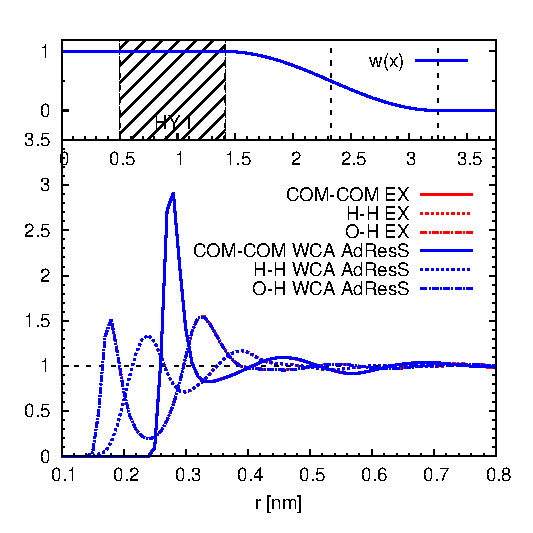
\includegraphics[width=0.6\textwidth]{fig/fig-rdf-all-wca-425-516.eps}
  \end{figure}
\end{frame}

\begin{frame}{WCA particles as a generic particle and energy reservior}
  {The accuracy: radiual distribution function}
  \begin{figure}
    \centering 
    \includegraphics[width=0.6\textwidth]{fig/fig-rdf-all-wca-516-608.eps}
  \end{figure}
\end{frame}

\begin{frame}{WCA particles as a generic particle and energy reservior}
  {The accuracy: radiual distribution function}
  \begin{figure}
    \centering 
    \includegraphics[width=0.6\textwidth]{fig/fig-rdf-all-wca-608-700.eps}
  \end{figure}
\end{frame}

\begin{frame}{WCA particles as a generic particle and energy reservior}
  {The accuracy: three-body correlation}
  \begin{figure}
    \centering 
    \includegraphics[width=0.95\textwidth]{fig/fig-wca-rdf3-diff-ex-hy1.eps}
  \end{figure}
\end{frame}


% \begin{frame}{WCA particles as a generic particle and energy reservior}
%   \begin{itemize}
%   \item<1-> Theoretically fist order accuracy
%   \item<2-> Numerically second order accuracy
%   \item<3-> Error of three-body correlation:
%   \begin{figure}
%     \centering 
%     \includegraphics[width=0.9\textwidth]{fig/fig-wca-rdf3-diff-ex-hy1.eps}
%   \end{figure}    
%   \end{itemize}
% \end{frame}


% \begin{frame}{Coarse-grained model: CG water v.s. WCA ``water''}
%   \small
%   \begin{table}
%     \centering
%     % \begin{tabular*}{0.9\textwidth}{@{\extracolsep{\fill}}lrr}
%     \begin{tabular}{l R{3cm} R{3cm}}
%       &         CG water &      WCA ``water'' \\\hline
%       \rowcolor{MyGray}
%       Efficiency &&\\
%       Cut-off \bluec{$r_c$} in nm     & \redc{0.90} & \bluec{0.34}\\
%       Computational expense:    & \redc{19}   & \bluec{1}\\
%       \rowcolor{MyGray}
%       $p(\vect x_\AT | N_\AT)$ & & \\
%       1st order: \bluec{$\rho_{\HY} = \rho_{\EX}$} & th. force \quad \bluec{\tickYes} & th. force \quad \bluec{\tickYes} \\
%       2st order: \bluec{$g_{\HY} = g_{\EX}$} & RDF corr.~\quad \bluec{\tickYes} & partially \quad \blackc{\tickYes}  \\
%       3rd order: \bluec{$\corr_{\HY} = \corr_{\EX}$} & numerically \quad \blackc{\tickYes} &  \redc{\tickNo} \\
%       \rowcolor{MyGray}
%       $p(N_\AT)$ &&\\
%       1st order: \bluec{$\mu_{\AT} = \mu_{\CG} - \omega_0$} & th. force \quad \bluec{\tickYes} & th. force \quad \bluec{\tickYes}\\
%       2nd order: \bluec{$\kappa_{\AT} = \kappa_{\CG}$}  & modelling \quad \bluec{\tickYes} & \redc{\tickNo}
%     \end{tabular}
%     % \end{tabular*}
%   \end{table}
% \end{frame}


\begin{frame}{AdResS vs. insertion particle method (IPM)}
  \vfill
    \centering
    \begin{tabular}{l|l|c|l}
      & Sys. size ($\textsf{nm}^3$)
      & Traj. (\textsf{ns})
      & CPU time (hours)\\    \hline
      AdResS   &$29.9\times3.7\times3.7$ & 1 & 3.1\\
      IPM & $3.7\times3.7\times3.7$ & 8 & 4.5 (traj.) + 36.7 (IPM)\\
    \end{tabular}
  
  \vfill
  \begin{itemize}
  \item<1-> IPM: \redc{Single insertion} at each test.\\
    $10^5 \textrm{(position)} \times 10^5 \textrm{(orientation)}$ test insertions every 0.2ps.\\
    Still not converged.
    \vfill
  \item<1-> AdResS: \redc{Multiple insertions}.\\
    23 trials per ps. 832 out of 13824 molecules inserted in 1ns.\\
    Thermodynamic equilibrium reached.
    \vfill
  \item<2-> Excess chemical potential of water: ($-23.5$ kJ/mol)\\
    AdResS: $-22.8$ kJ/mol (3.0\%)\\
    IPM: \ \quad$-24.6$ kJ/mol (4.7\%) (400 ns traj. !)
  \end{itemize}
  % \caption{Comparison of computational efficiency.
  %     The AdResS simulation contains 13824 molecules, while the full atomistic (EX)
  %     water simulations contain 1728 molecules. In the AdResS simulation,
  %     the size of the AT + HY regions ($6.7\times3.7\times3.7\textsf{nm}^3$) is even larger than that of the EX water
  %     simulation box, so that we are actually in a {\it ``worst scenario''} situation. Moreover simulations with smaller reservoirs  gave essentially the same results reported for this system.
  %     ``Sys. size'' means the size of the box used in the simulation.
  %     ``Traj. length'' means the equilibrium trajectory
  %     used for the particle insertion in the IPM approach. Along the trajectories, frames
  %     of configurations were recorded every 0.2~\textsf{ps}.
  %     ``CPU time'' the is wall clock time spend on the simulation.
  %     For the particle insertion simulation, the CPU time is counted by two
  %     parts: the time of generating the equilibrium trajectories (traj.) (not expensive)
  %     and the time required by the IPM procedure (very expensive). Moreover, not only the insertion procedure is expensive on itself, but even after $8\textsf{ns}$ the insertion process has not actually converged. Simulations on longer time scales show that the full convergence is actually never reached, which suggests that the insertion procedure for a molecule as simple as water is not fully rigorous from the physical point of view.
  %   }
\end{frame}


\begin{frame}{The solvation free energy of mixtures}{Schematic plot of the system urea solved in water}
  \begin{figure}
    \centering
    \includegraphics[width=0.995\textwidth]{fig/system.mix/system.eps}
  \end{figure}
  The chemical potential of the component:
  \bluec{
    \begin{align*}
      \mu^{\textrm{solute}}_\AT &= \mu^{\textrm{solute}}_\CG - \omega^{\textrm{solute}}_0\\
      \mu^{\textrm{solvent}}_\AT &= \mu^{\textrm{solvent}}_\CG - \omega^{\textrm{solvent}}_0
    \end{align*}
  }
\end{frame}


\begin{frame}{The solvation free energy of mixtures}
  {The numbers are in unit kJ/mol}
  \vfill
  \begin{table}
    \centering
    % \begin{tabular*}{0.9\textwidth}{@{\extracolsep{\fill}}rrrrr}
    \begin{tabular}{rr  R{2cm} R{2cm} R{2cm}}
      Solute & Solvent & AdResS &
      T.I.$^1$ &
      Experiment$^1$  \\
      \hline
      methane & water  & 10.3 & 8.7 & 8.4 \\
      \rowcolor{MyGray}
      methanol & water  & $-18.9$ & $-22.1$ & $-21.2$ \\
      urea &water  & $-54.6$ & $-60.9$ & $-57.5$ \\
      \rowcolor{MyGray}
      methane & methanol & 3.2 & 3.2 & 1.6 \\
      methanol & methanol & $-19.4$ & $-25.0$ & $-20.5$  
    \end{tabular}
  \end{table}
  \vfill
  \footnotesize{1. D.P. Geerke and W.F. van Gunsteren, ChemPhysChem, \textbf{7} (2006)}
\end{frame}


\begin{frame}{Force interpolation v.s. potential interpolation}
  \begin{itemize}
  \item <1-> Force interpolation:
    \bluec{
      \begin{equation*}
        {\vect F}_{\alpha \beta}=w_\alpha w_\beta{\vect F}_{\alpha\beta}^{\AT}+[1-w_\alpha w_\beta]{\vect F}^{\CG}_{\alpha\beta}       
      \end{equation*}
    }
  \item <2-> Potential interpolation:
    \bluec{
      \begin{equation*}
        {V}_{\alpha \beta}=w_\alpha w_\beta{V}_{\alpha\beta}^{\AT}+[1-w_\alpha w_\beta]{V}^{\CG}_{\alpha\beta}        
      \end{equation*}
    }
  \item <3-> The force of potential AdResS:
    \bluec{
      \begin{align*}
        {\vect F}^V_{\alpha \beta}&= -\nabla_{\alpha}{V}_{\alpha \beta} \\
        &=w_\alpha w_\beta{\vect F}_{\alpha\beta}^{\AT}+[1-w_\alpha w_\beta]{\vect F}^{\CG}_{\alpha\beta}  - \redc{\nabla w_\alpha\cdot w_\beta (V^\AT_{\alpha \beta} - V^\CG_{\alpha \beta})}
      \end{align*}
    }
  \item <4-> The force of changing representation:
    \bluec{
      \begin{equation*}
        {\vect F}^{\rep}_\alpha = \sum_\beta \nabla w_\alpha \cdot w_\beta (V^\AT_{\alpha \beta} - V^\CG_{\alpha \beta})
      \end{equation*}
    }
  \end{itemize}
\end{frame}



\begin{frame}{The equilvance of the two approachs}
  \begin{itemize}\itemsep -1.0cm
  \item <1-> Calculate the thermodynamic force for both approachs.\\
    The total force on molecule $\alpha$:
    \bluec{
      \begin{align*}
        \vect F_\alpha &= \sum_\beta \vect F_{\alpha\beta} + \vect F^\thf_\alpha\\
        \vect F^V_\alpha &= \sum_\beta \vect F_{\alpha\beta} + \vect F^{\thf,V}_\alpha - \vect F_\alpha^\rep\\
      \end{align*}
    }
  %       % {\vect F}_{\alpha} = {\vect F}^V_{\alpha} - {\vect F}^\rep_{\alpha}
  % \item <2-> Calculate the thermodynamic force \bluec{$\vect F^{\thf,P}_\alpha$} for the potential AdResS:
  %   \bluec{
  %     \begin{align*}
  %       \int \vect F^\thf_{\alpha} d\vect x = \int{\vect F}^{\thf,P}_{\alpha}d \vect x
  %       - \int \langle{\vect F}^\rep_{\alpha}\rangle d \vect x
  %     \end{align*}      
  %   }
  \item <2-> Let  \bluec{$\Delta \vect F^\thf = \vect F^{\thf,V} - \vect F^\thf
      \,=\, \redc{\mathlarger{\mathlarger{\langle \vect F^\rep \rangle}}}$}
  \begin{figure}
    \centering 
    \includegraphics[width=0.5\textwidth]{fig/fig-diff-thf.eps}
  \end{figure}      
  \end{itemize}
\end{frame}

\begin{frame}{What are the differences}
  \small{
  \begin{table}
    \centering
    \begin{tabular*}{0.95\textwidth}{@{\extracolsep{\fill}}lll}
      &         Force interp. AdResS     &       Potential interp. AdResS \\\hline
      Momentum consv.     &       \bluec{\tickYes}        &       \redc{\tickNo}\\      
      \rowcolor{MyGray}
      Energy consv. &     \redc{\tickNo}  &       \bluec{\tickYes}\\
      th. force &  \bluec{\tickYes} &  \bluec{\tickYes}\\
      \rowcolor{MyGray}
      RDF corr. &  \bluec{\tickYes} &  \redc{\tickNo}\\
      Temperture          &     \bluec{$T_{target}$}      & \bluec{$T_{target}$}\\
      \rowcolor{MyGray}
      Pressure          &   \bluec{$p_\AT = p_\CG - \rho_0\, \omega^\thf$} &
      \bluec{$p_\AT = p_\CG - \rho_0\, (\omega^\thf - \omega^\rep)$}\\
      Chemical potentail          &   \bluec{$\mu_\AT = \mu_\CG - (\omega^\thf +\omega^\rep)$} &
      \bluec{$\mu_\AT = \mu_\CG - \omega^\thf$}
    \end{tabular*}
  \end{table}
  }
\end{frame}


\begin{frame}{Acknowledgement}
  \vfill
  The authors:
  \begin{itemize}
  \item Luigi Delle Site (Freie Universit\"at Berlin)
  \item Carsten Hartmann (Freie Universit\"at Berlin)
  \item Christof Sch\"utte (Freie Universit\"at Berlin \& Zuse Institute Berlin)
  \end{itemize}
  \vfill
  For more details:
  \begin{itemize}
  \item H. Wang, C. Hartmann, C. Sch\"utte and L. Delle Site,\\
    \textbf{Phys. Rev. X}, 3, 011018, (2013).
  \item H. Wang, C. Sch\"utte and L. Delle Site,\\
    \textbf{J. Chem. Theory \& Compt.}, 8(8), 2878-2887 (2012).
  \end{itemize}
  \vfill
\end{frame}

\begin{frame}[plain]
  \vfill
  \begin{figure}
    \centering 
    \includegraphics[width=0.88\textwidth]{fig/system.cover/main.eps}
  \end{figure}
  \vskip -.5cm
  \footnotesize{
    1, Phys. Rev. X, 3, 011018, (2013).\\
  \vskip -.1cm
    2, J. Chem. Theory \& Compt., 8(8), 2878-2887 (2012).
  }
\end{frame}

\appendix

\begin{frame}{Numerical verification}{Density profile}
  \begin{figure}
    \centering 
    \includegraphics[width=0.8\textwidth]{fig/fig-rho.eps}
  \end{figure}  
\end{frame}

\begin{frame}{Numerical verification}{Fluctuation}
  \begin{figure}
    \centering 
    \includegraphics[width=0.8\textwidth]{fig/fig-count.eps}
  \end{figure}  
\end{frame}

\begin{frame}{Numerical verification}{RDFs}
  \begin{figure}
    \centering 
    \includegraphics[width=0.6\textwidth]{fig/fig-rdf-all-375-425.eps}
  \end{figure}  
\end{frame}

\begin{frame}{Numerical verification}{RDFs}
  \begin{figure}
    \centering 
    \includegraphics[width=0.6\textwidth]{fig/fig-rdf-all-425-516.eps}
  \end{figure}  
\end{frame}

\begin{frame}{Numerical verification}{RDFs}
  \begin{figure}
    \centering 
    \includegraphics[width=0.6\textwidth]{fig/fig-rdf-all-516-608.eps}
  \end{figure}  
\end{frame}

\begin{frame}{Numerical verification}{RDFs}
  \begin{figure}
    \centering 
    \includegraphics[width=0.6\textwidth]{fig/fig-rdf-all-608-700.eps}
  \end{figure}  
\end{frame}


\begin{frame}{Numerical verification}{Three-body correlation}
  \begin{figure}
    \centering 
    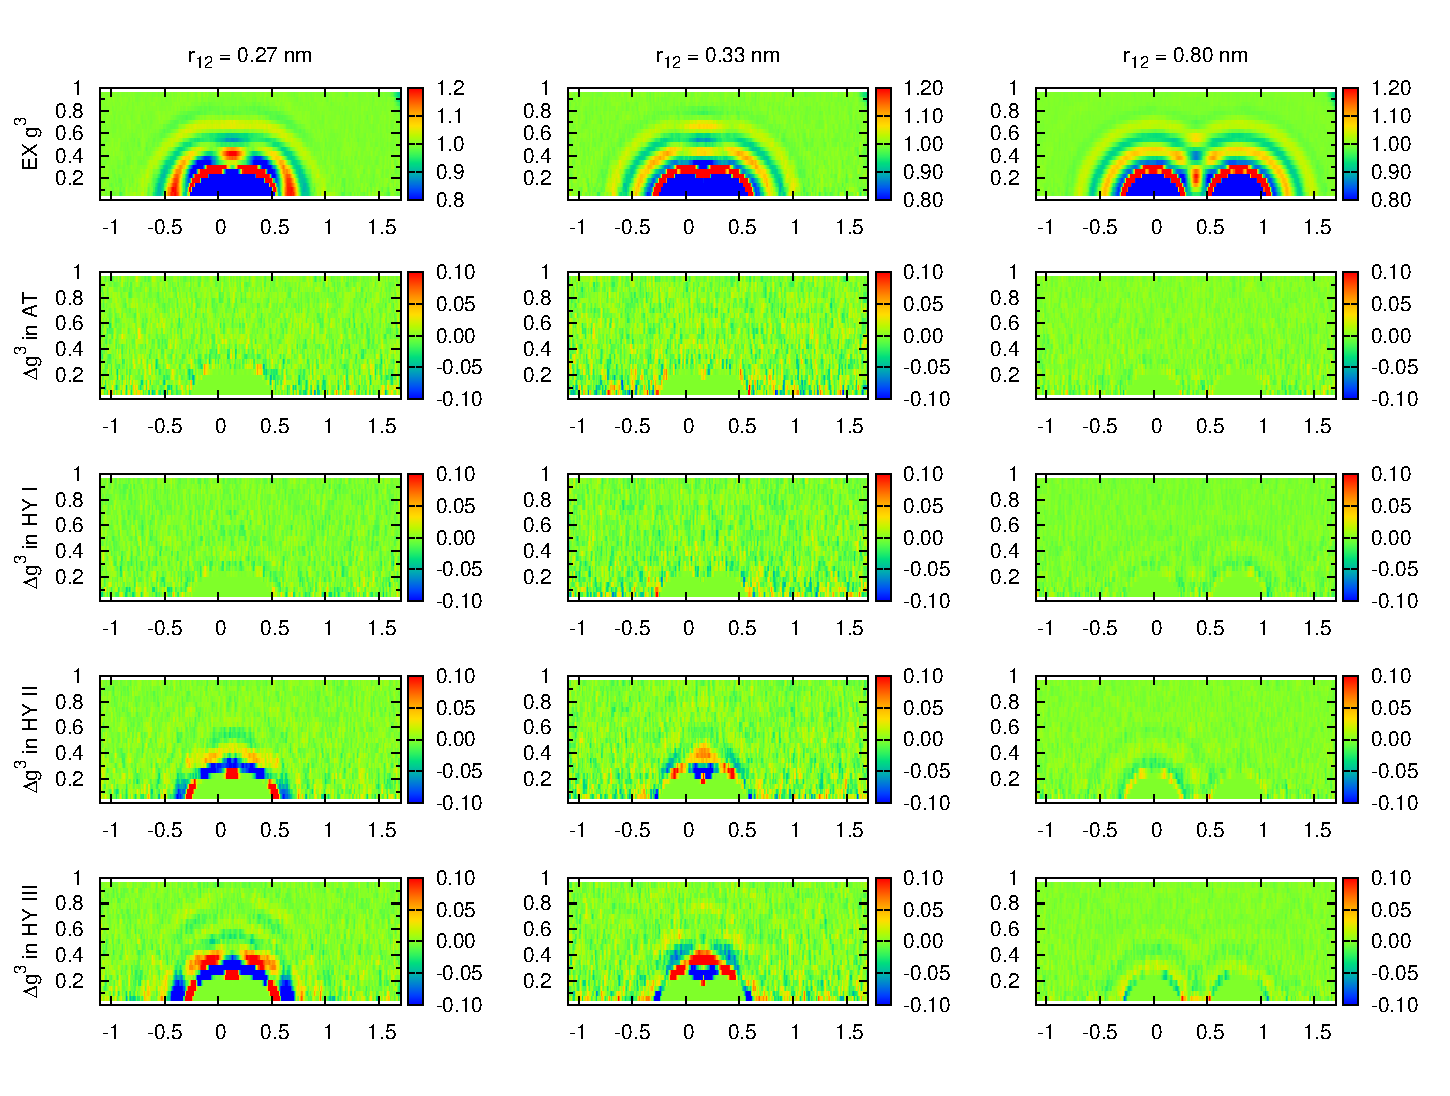
\includegraphics[width=0.9\textwidth]{fig/fig-rdf3-diff.eps}
  \end{figure}  
  Definition
  \tiny{\bluec{
    \begin{align*}
      \corr (\vect s_1, \vect s_2, \vect s_3)
      =
      \frac1{\rho(\vect s_1)\rho(\vect s_2)\rho(\vect s_3)}
      \big\langle
      (\hat\rho(\vect s_1) - \rho(\vect s_1))\cdot
      (\hat\rho(\vect s_2) - \rho(\vect s_2))\cdot
      (\hat\rho(\vect s_3) - \rho(\vect s_3))
      \big\rangle
    \end{align*}}}
\end{frame}

\begin{frame}{Convergence of the IPM}
  \begin{figure}
    \centering 
    \includegraphics[width=0.8\textwidth]{fig/fig-tpi.eps}
  \end{figure}  
\end{frame}



\end{document}
